\begin{figure*}
\centering
\subfloat[\label{fig:accuracy-mlalgos-time16} N=16]{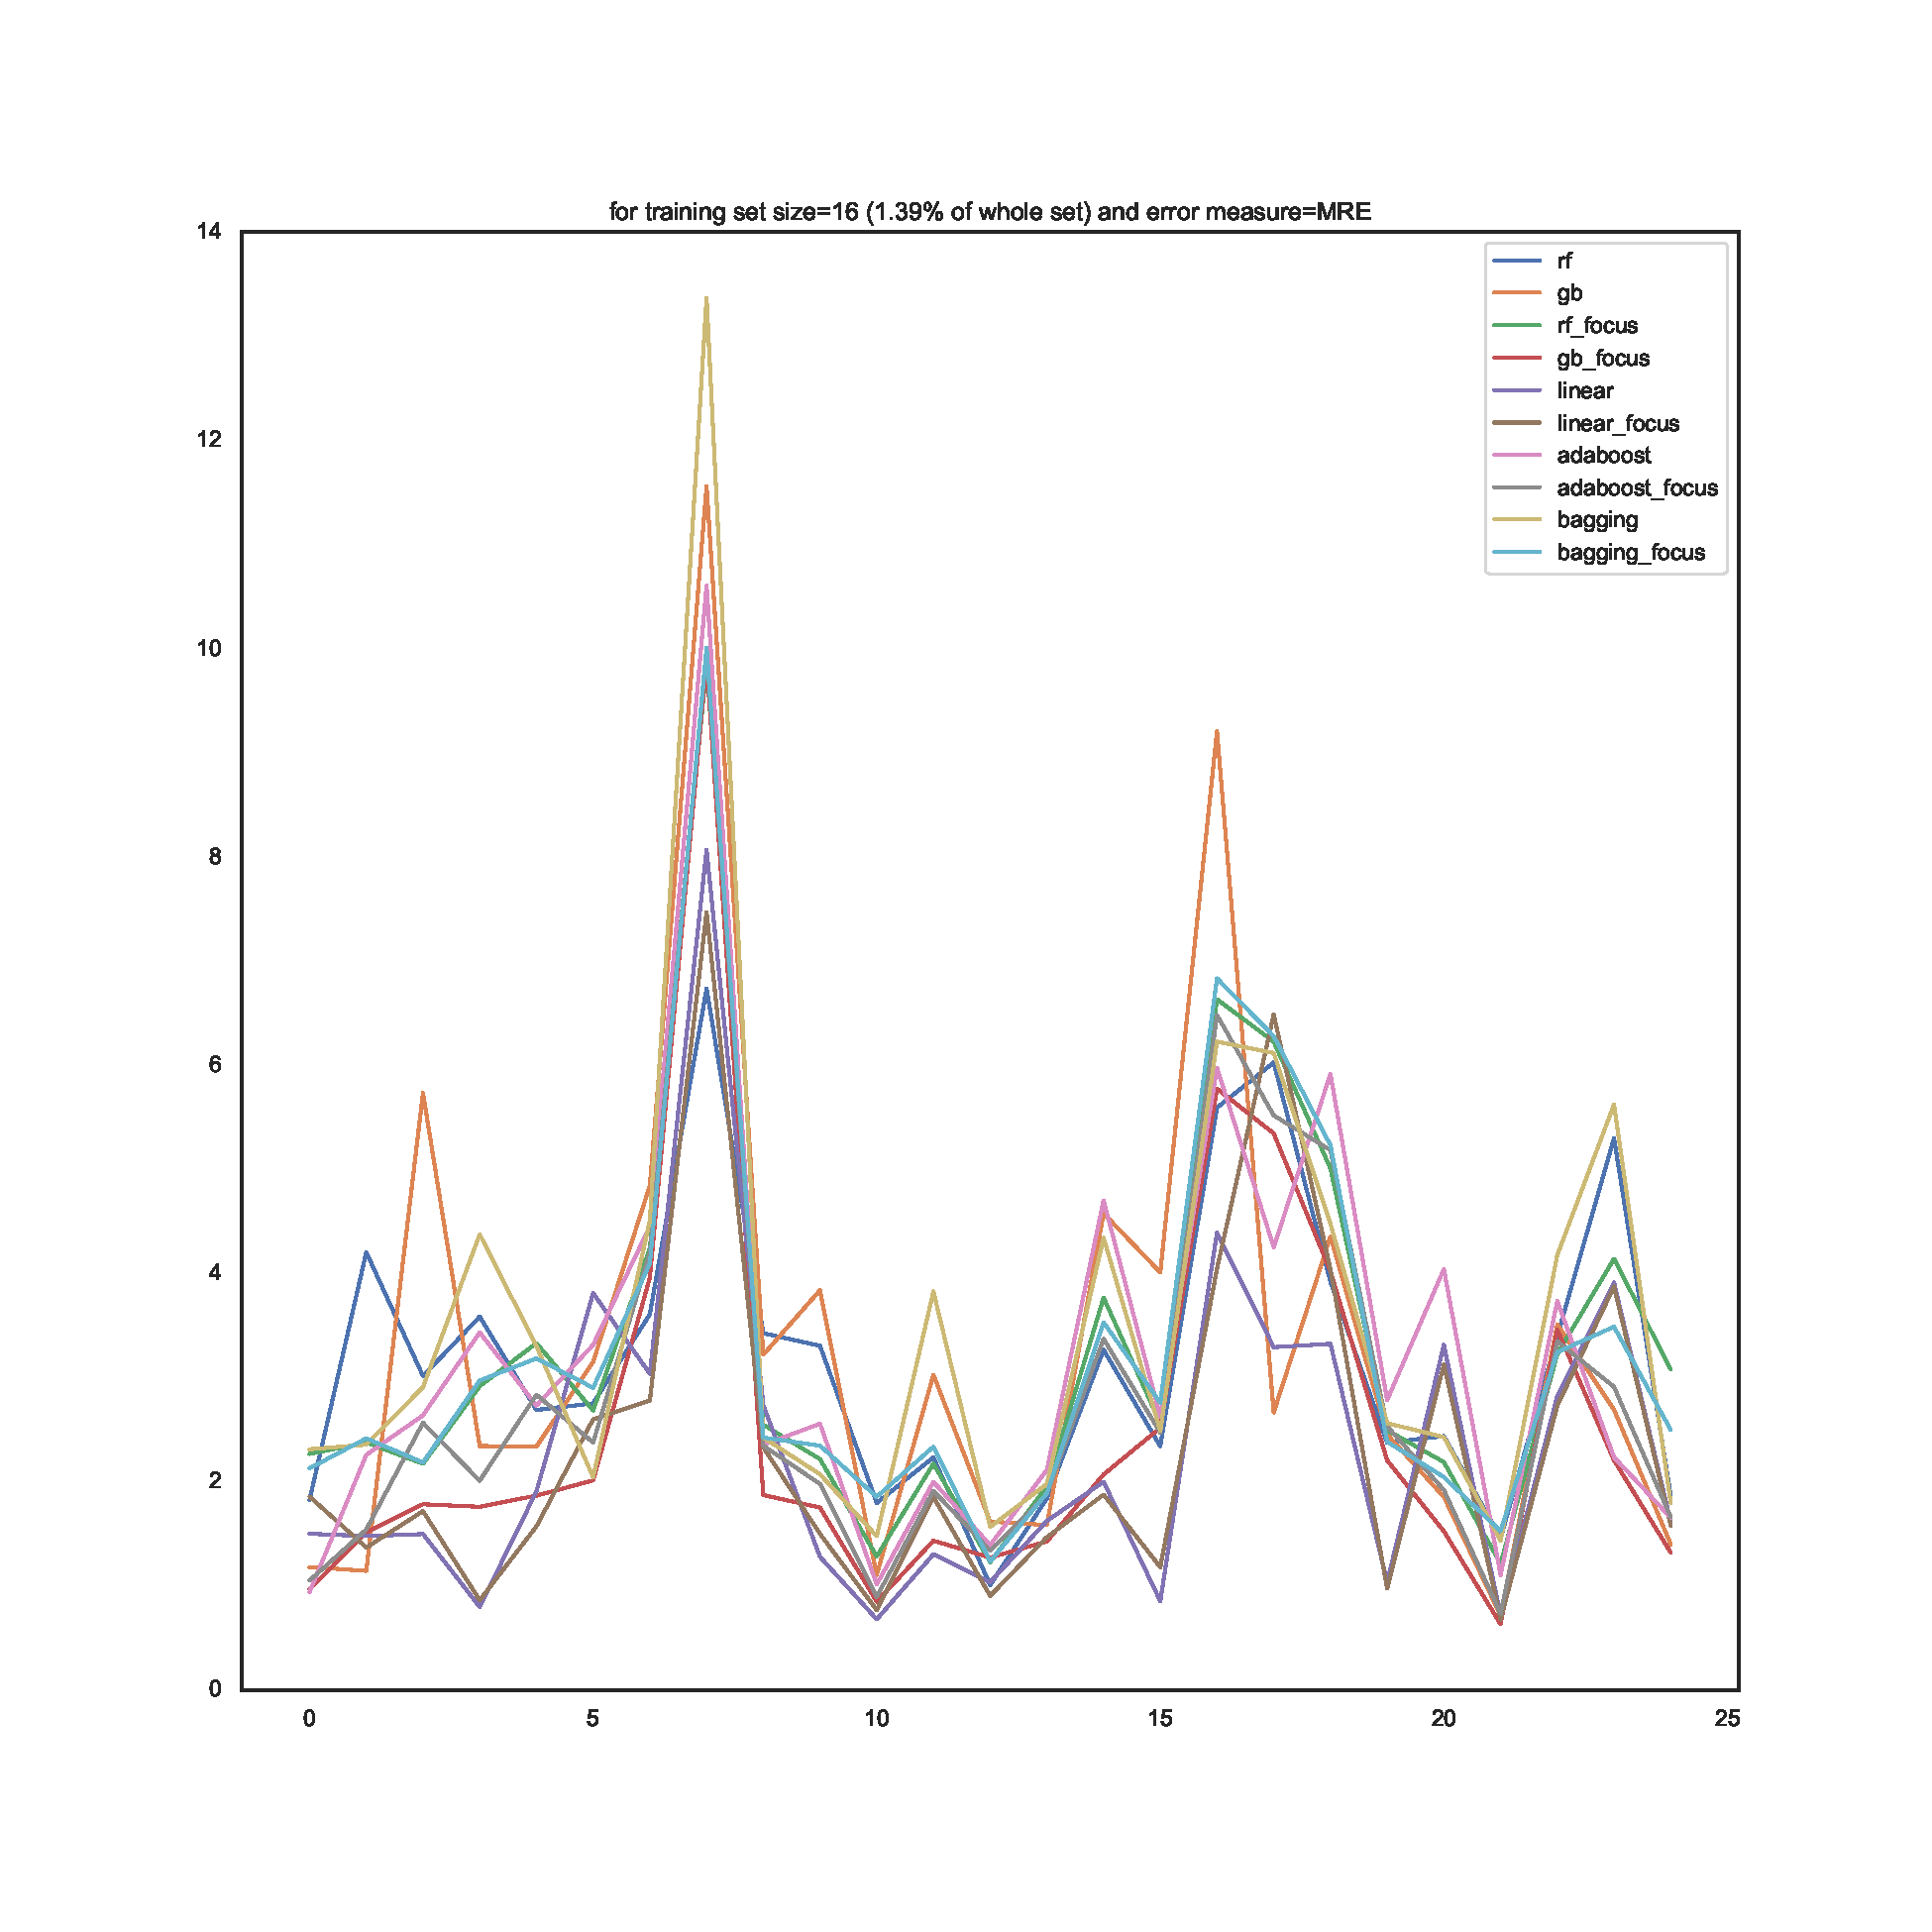
\includegraphics[scale=0.12]{JupyterImages/focuseffect_evo_16_MRE-size.pdf}}
\subfloat[\label{fig:accuracy-mlalgos-time32} N=32]{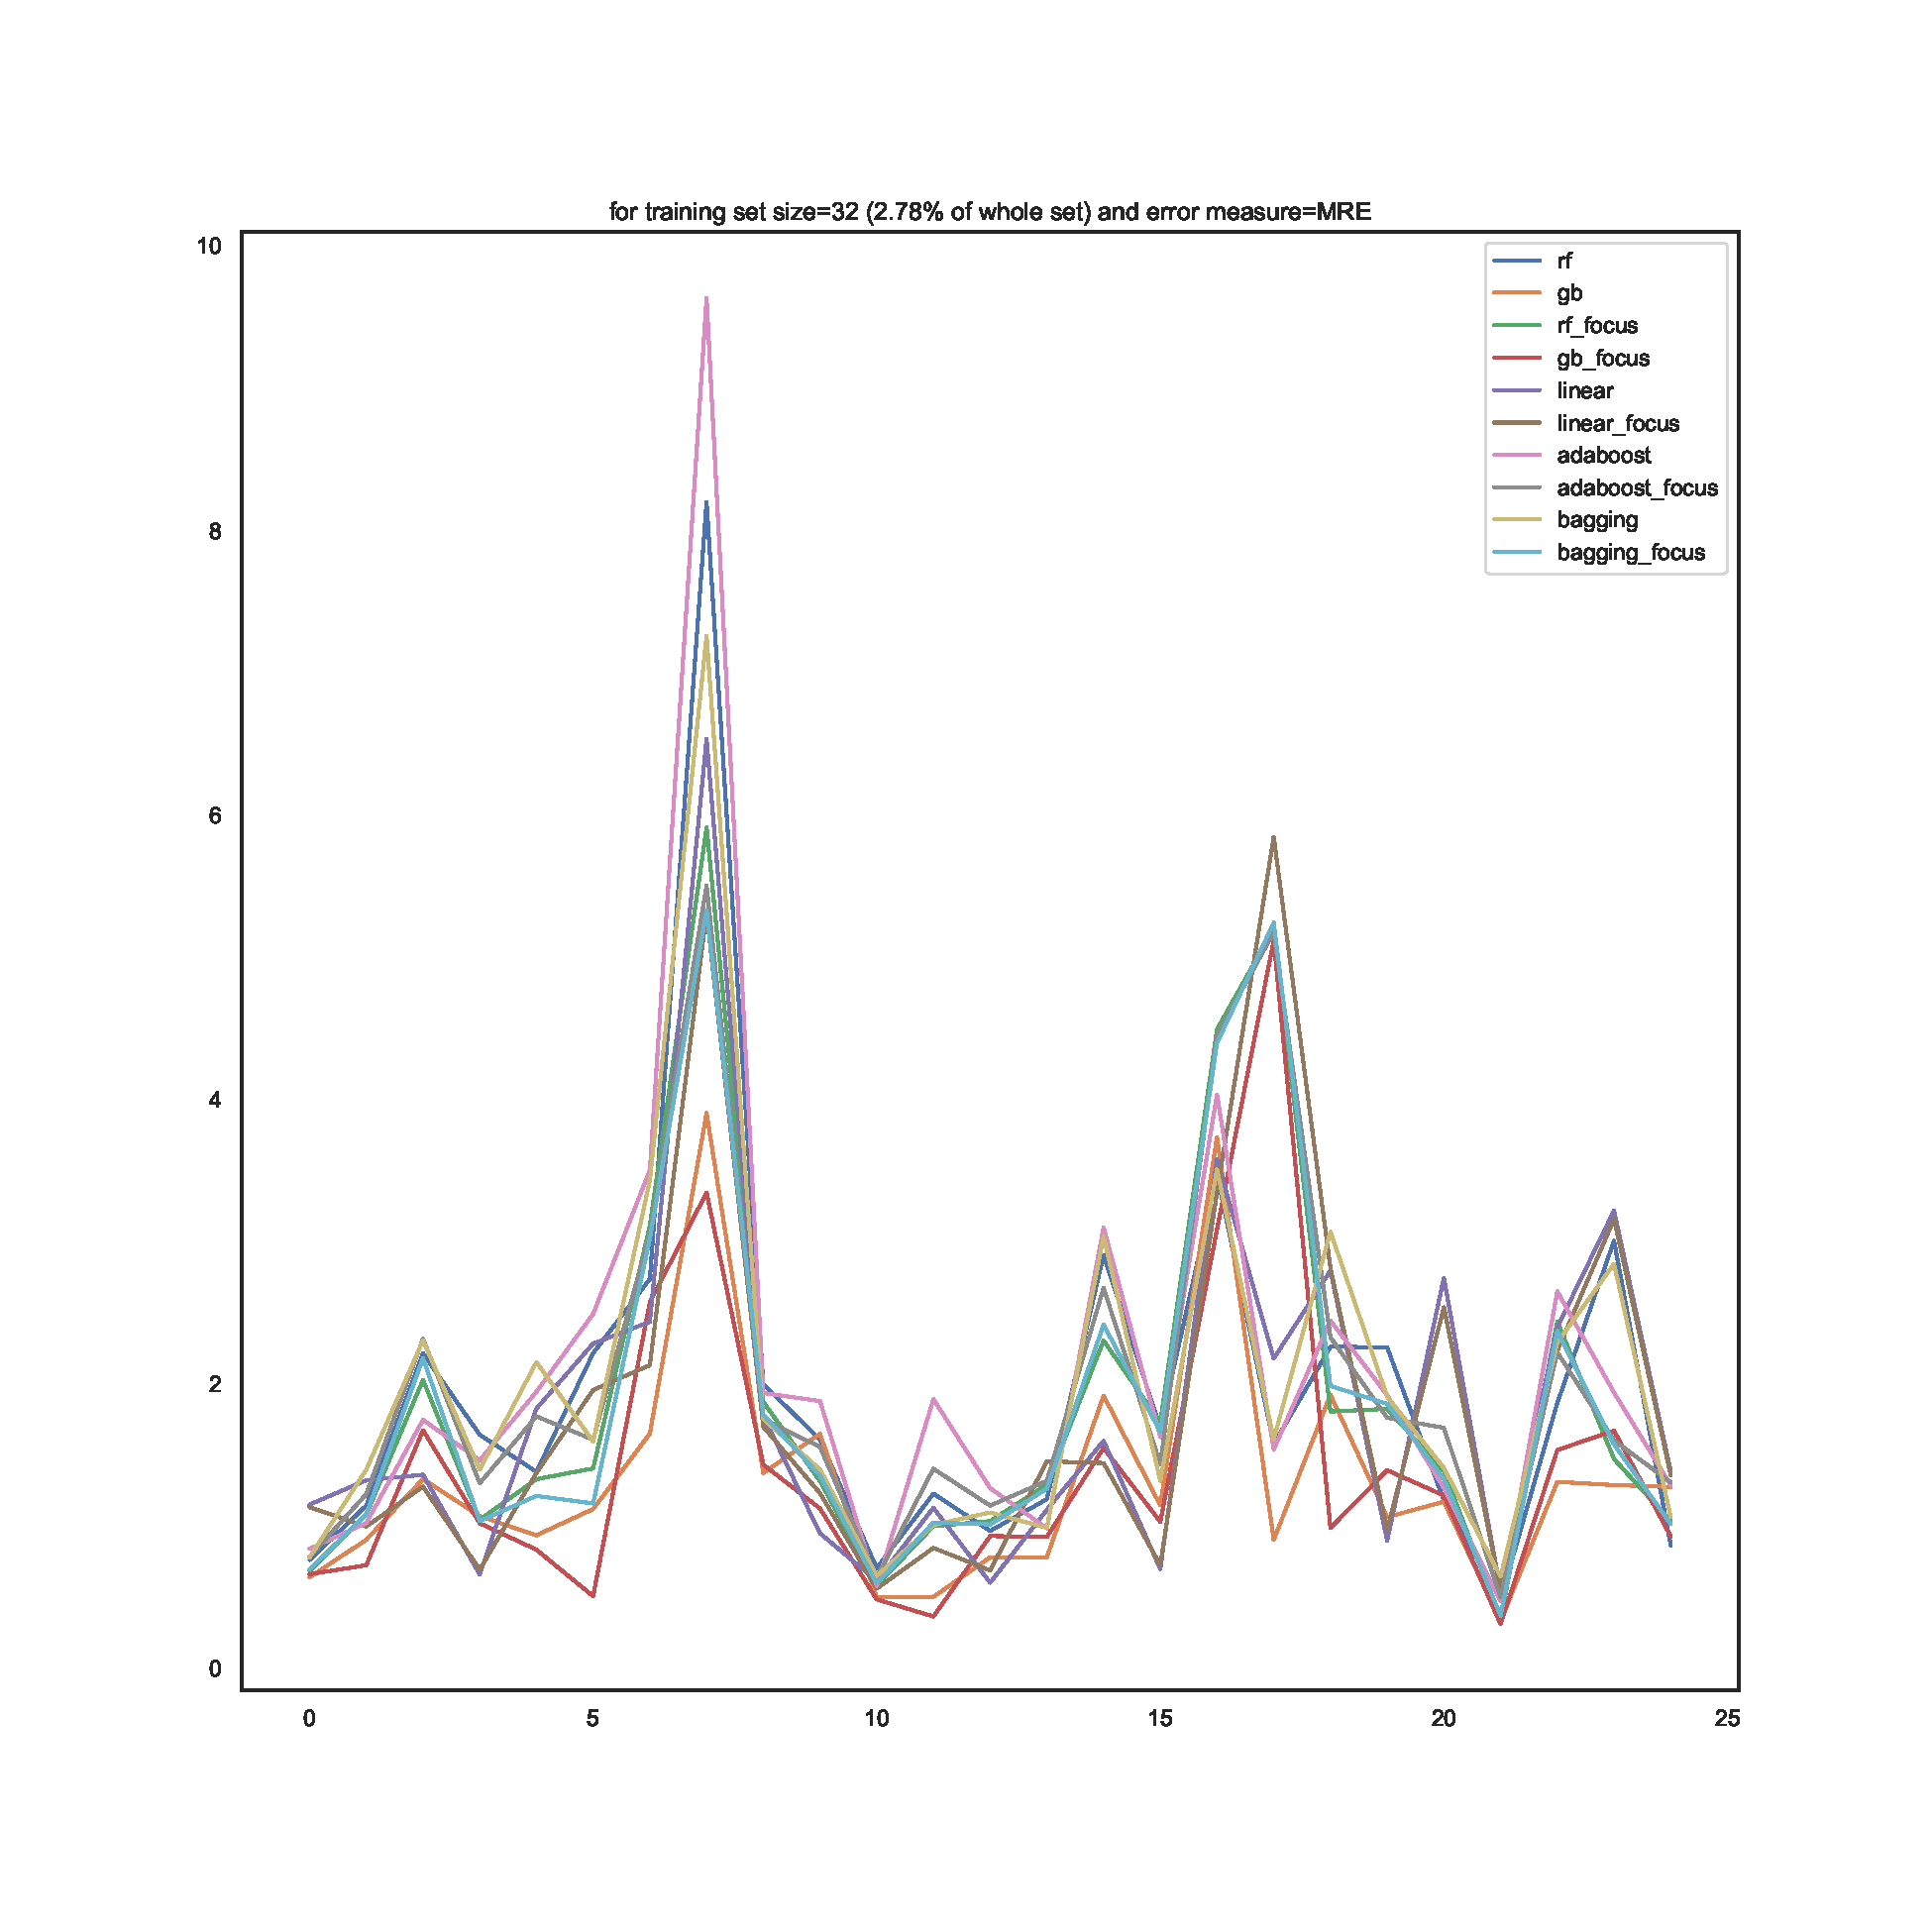
\includegraphics[scale=0.12]{JupyterImages/focuseffect_evo_32_MRE-size.pdf}}\\
\subfloat[\label{fig:accuracy-mlalgos-time48} N=48]{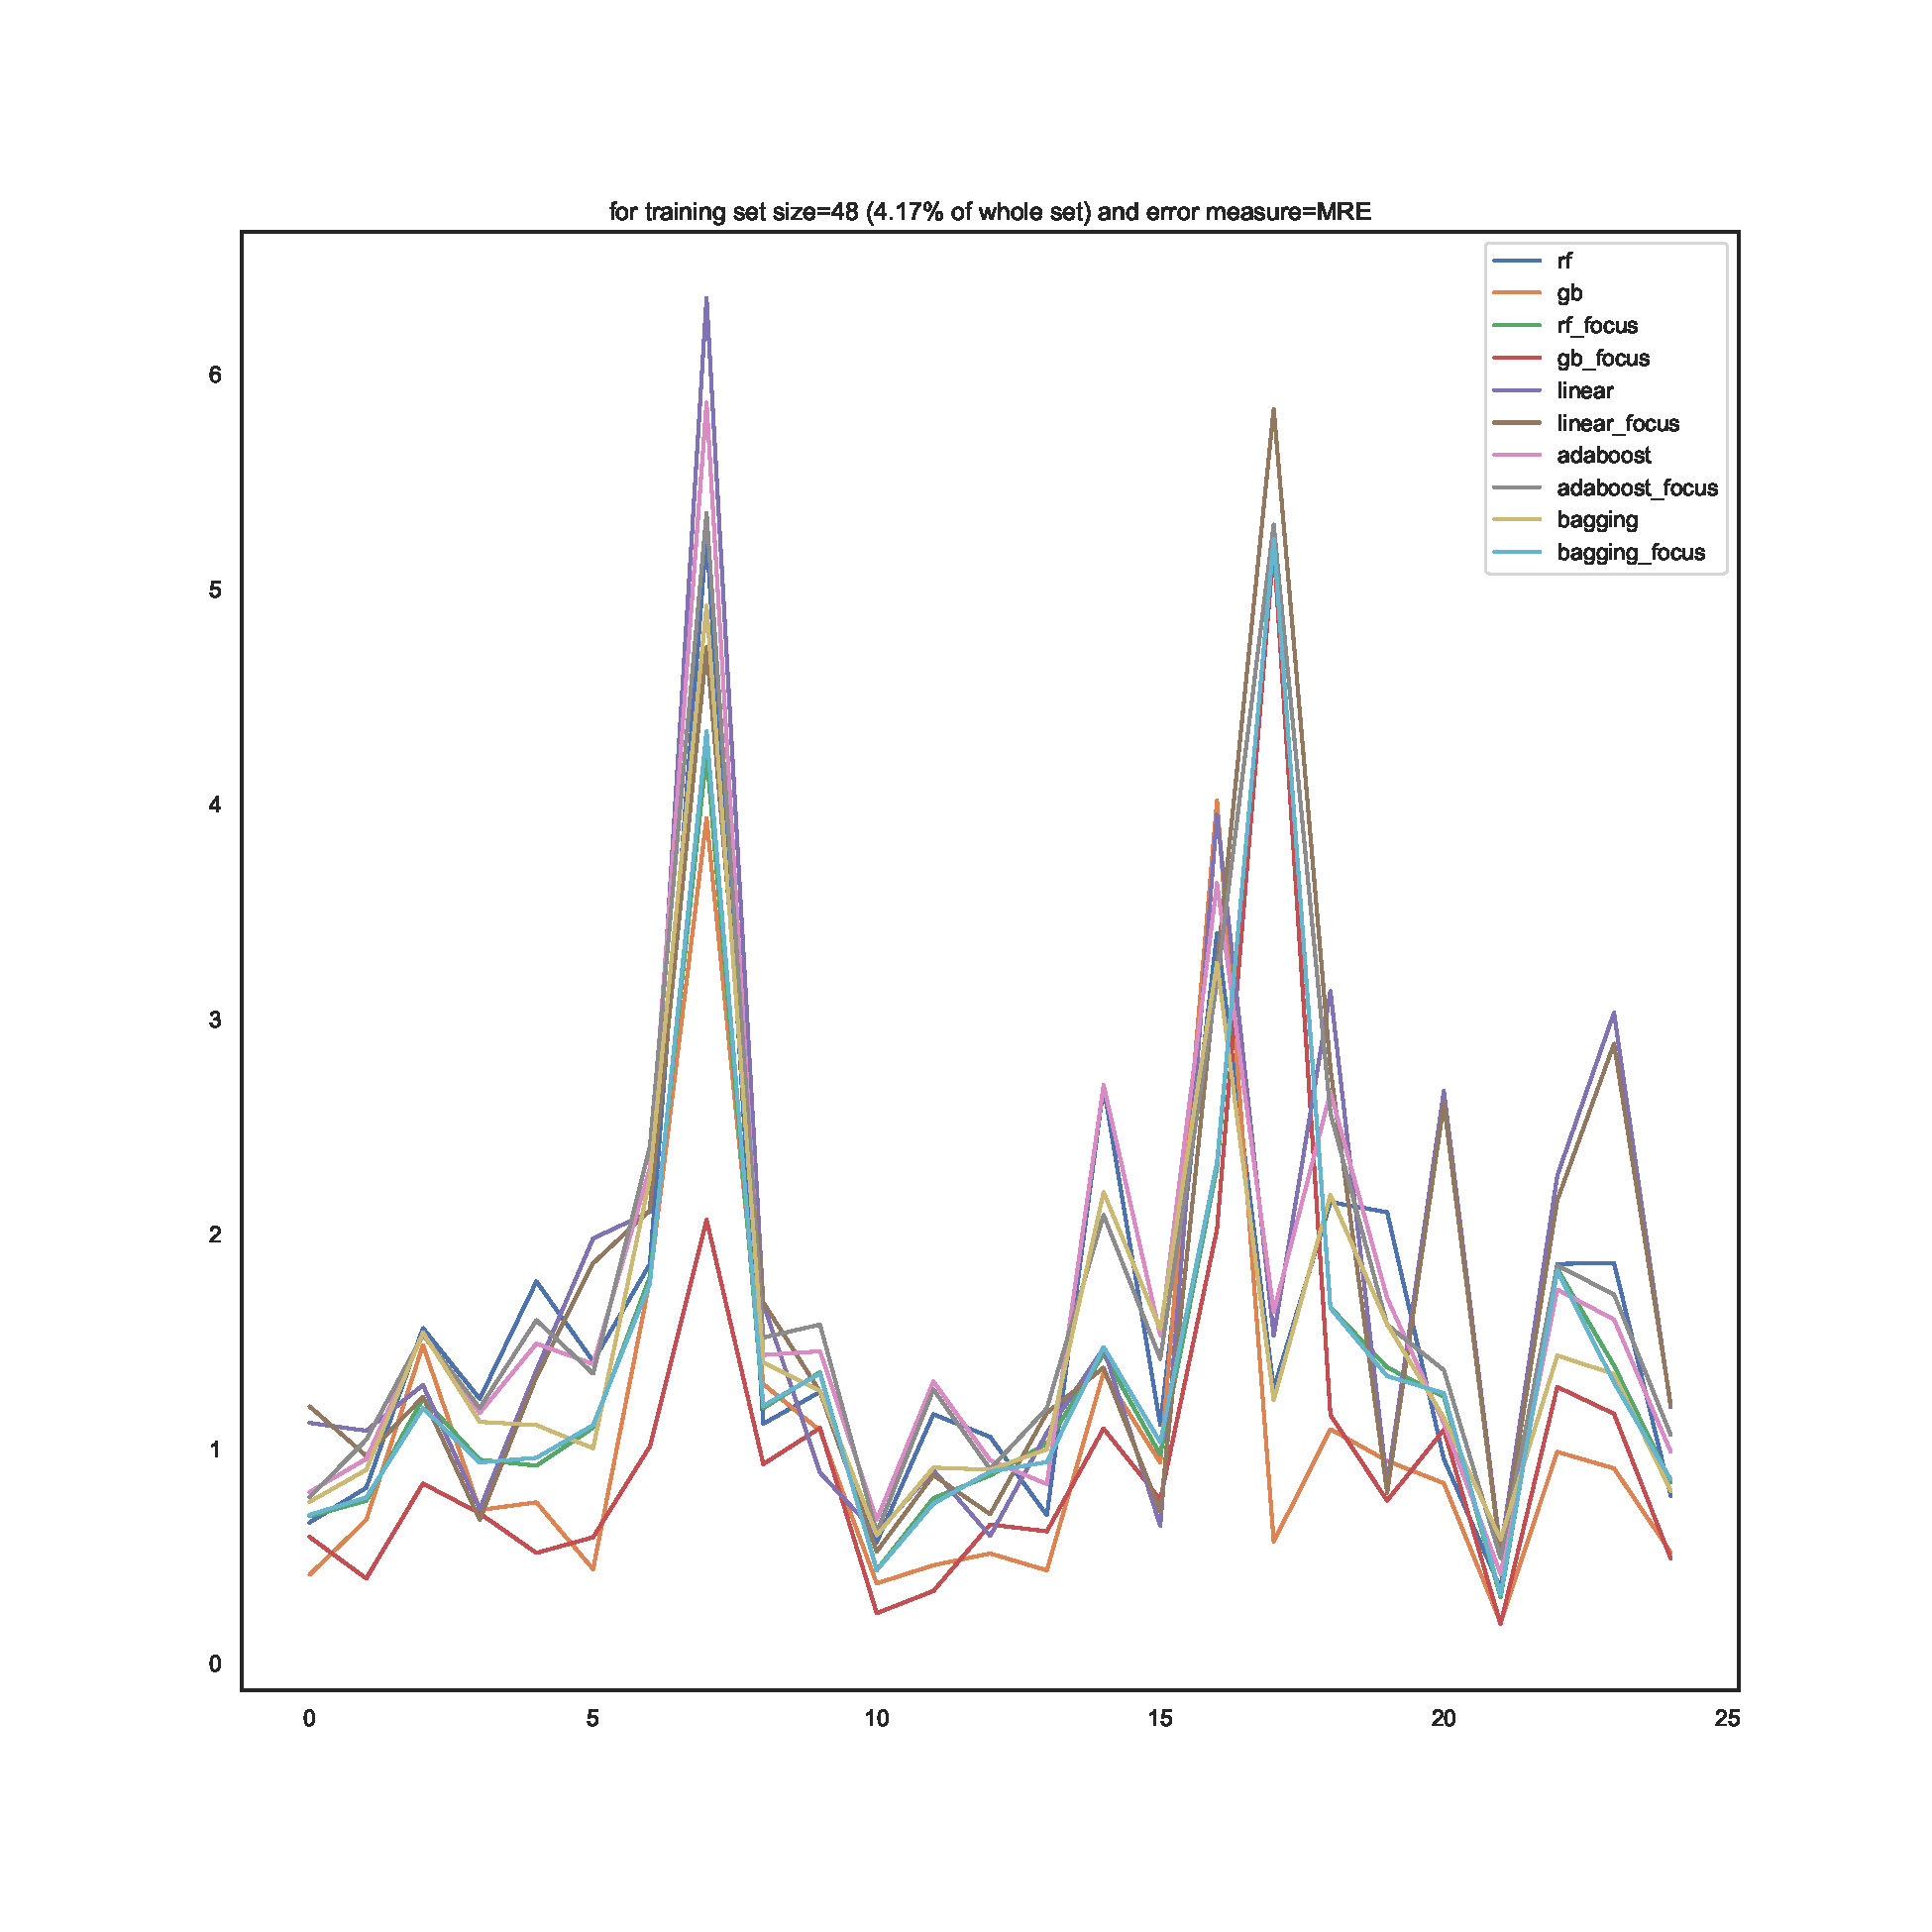
\includegraphics[scale=0.12]{JupyterImages/focuseffect_evo_48_MRE-size.pdf}}
\subfloat[\label{fig:accuracy-mlalgos-time64} N=64]{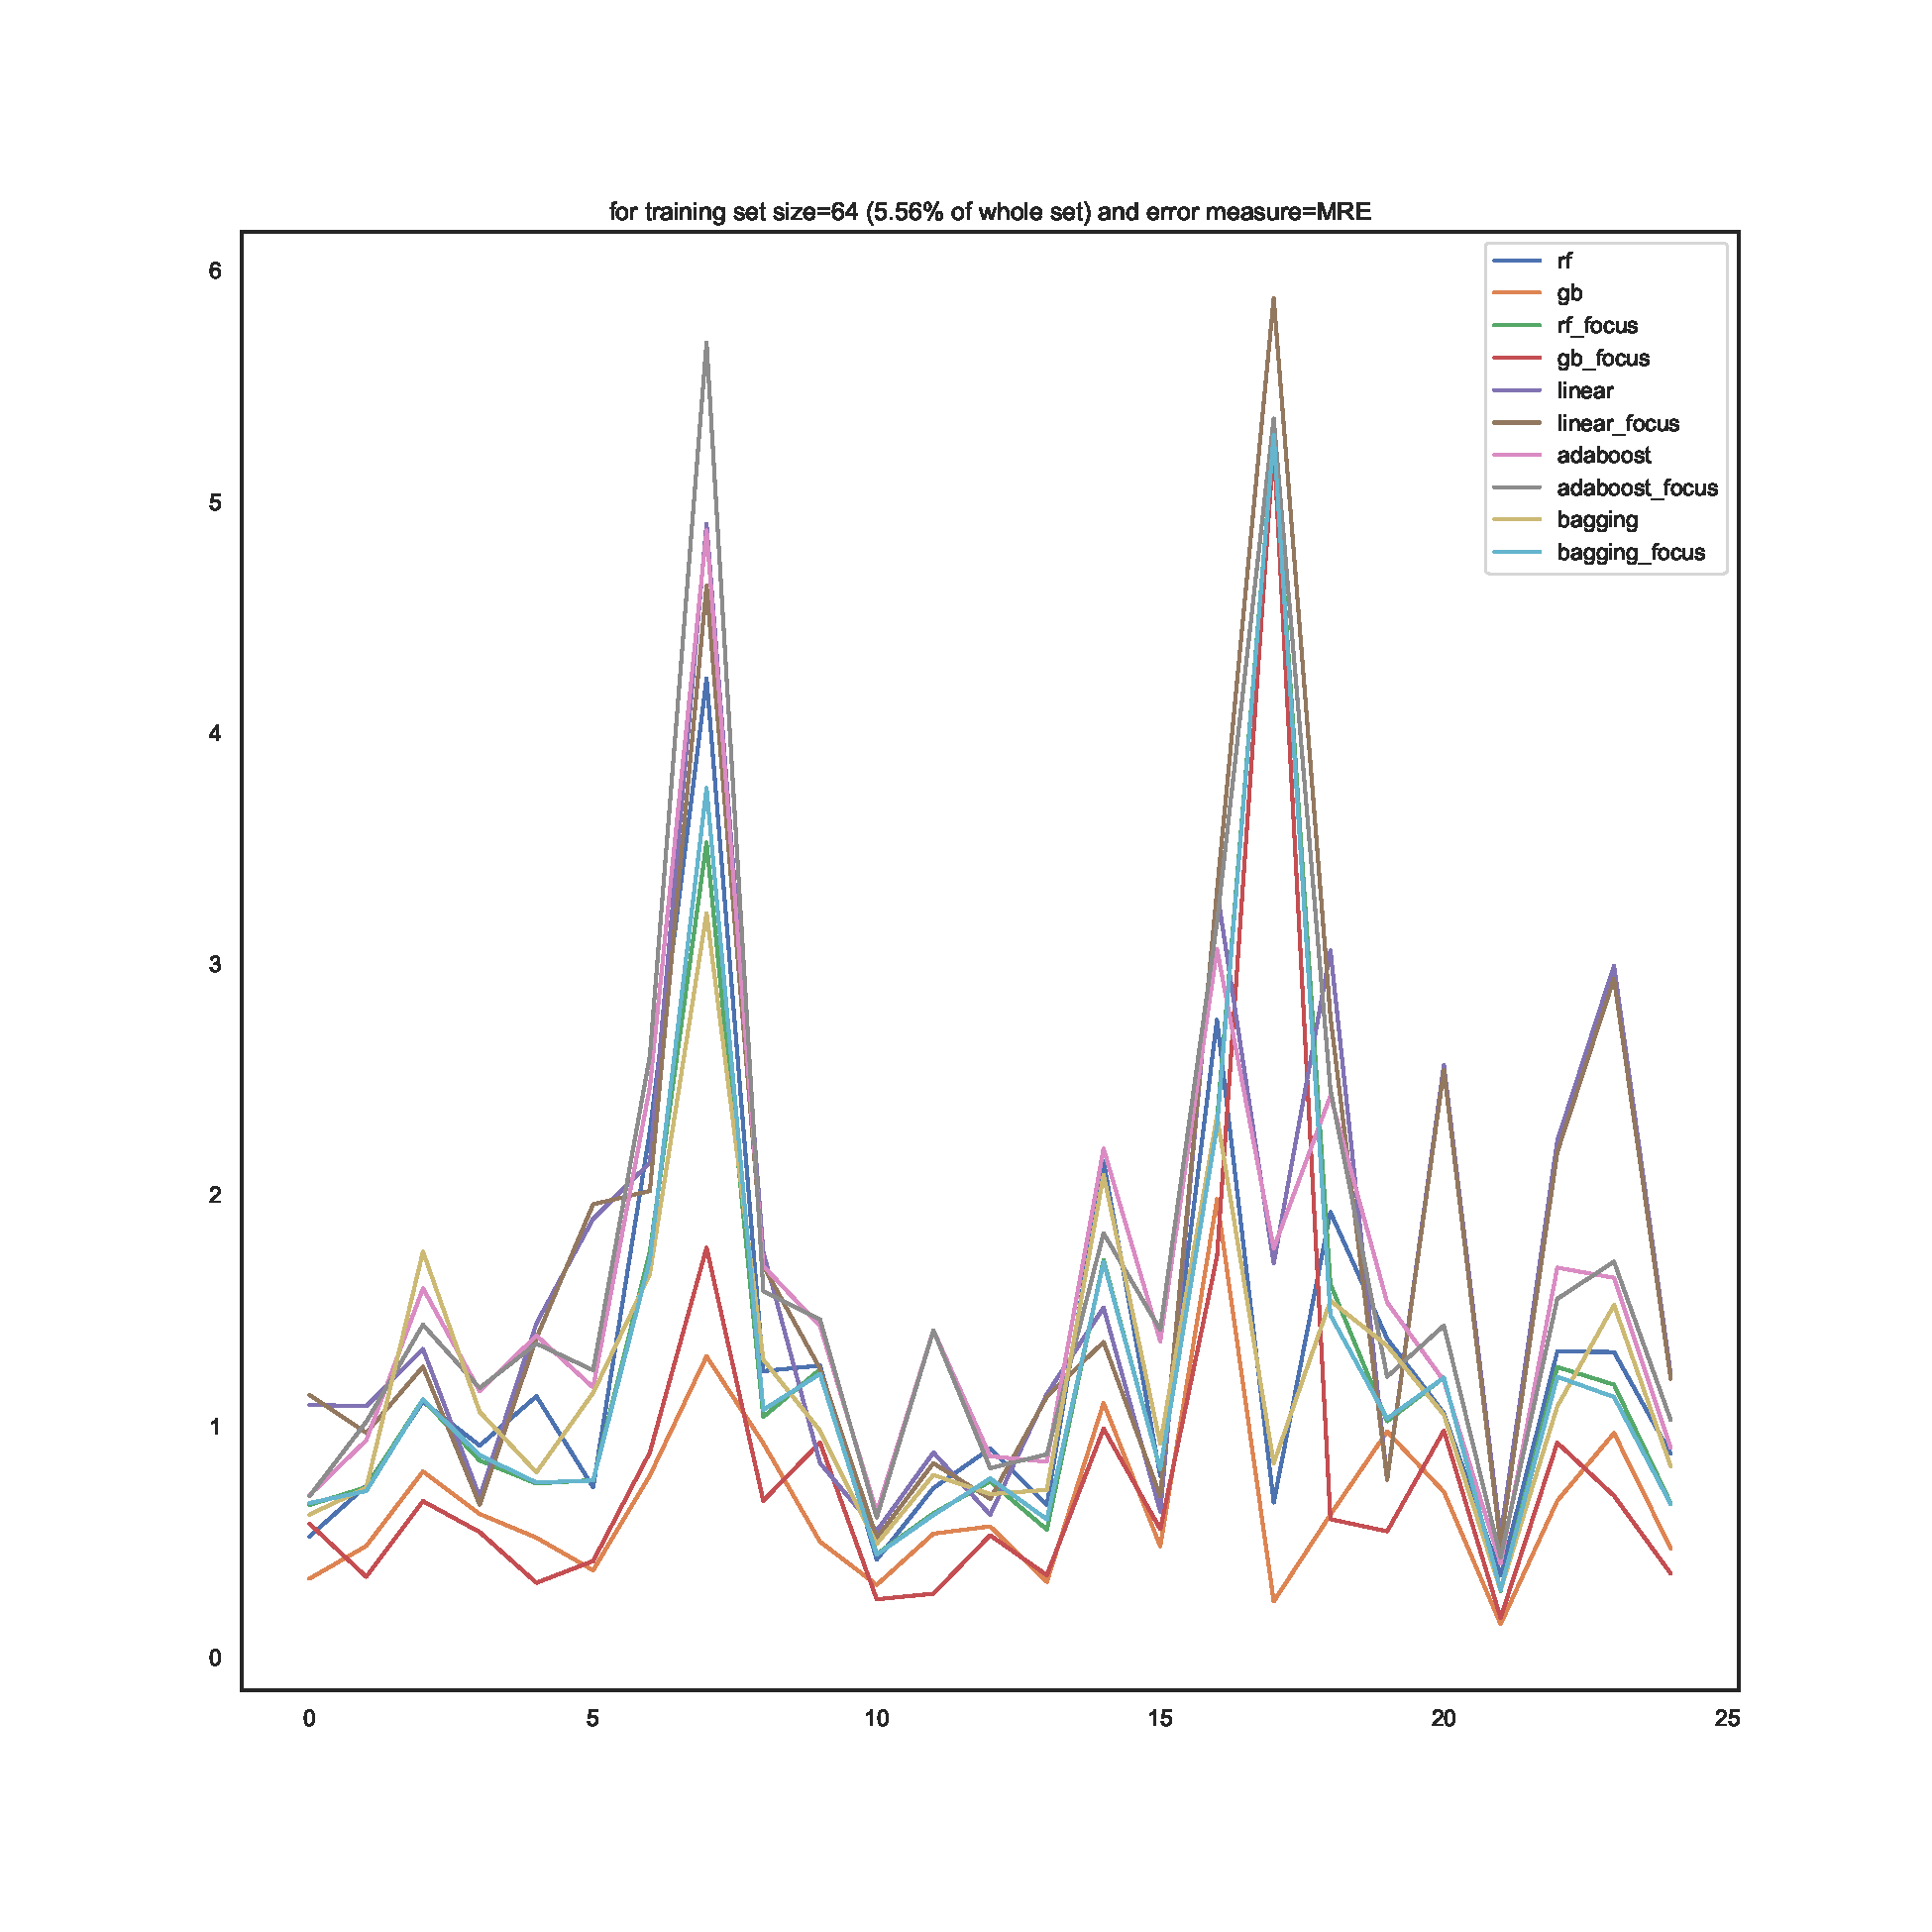
\includegraphics[scale=0.12]{JupyterImages/focuseffect_evo_64_MRE-size.pdf}}\\
\subfloat[\label{fig:accuracy-mlalgos-time80} N=80]{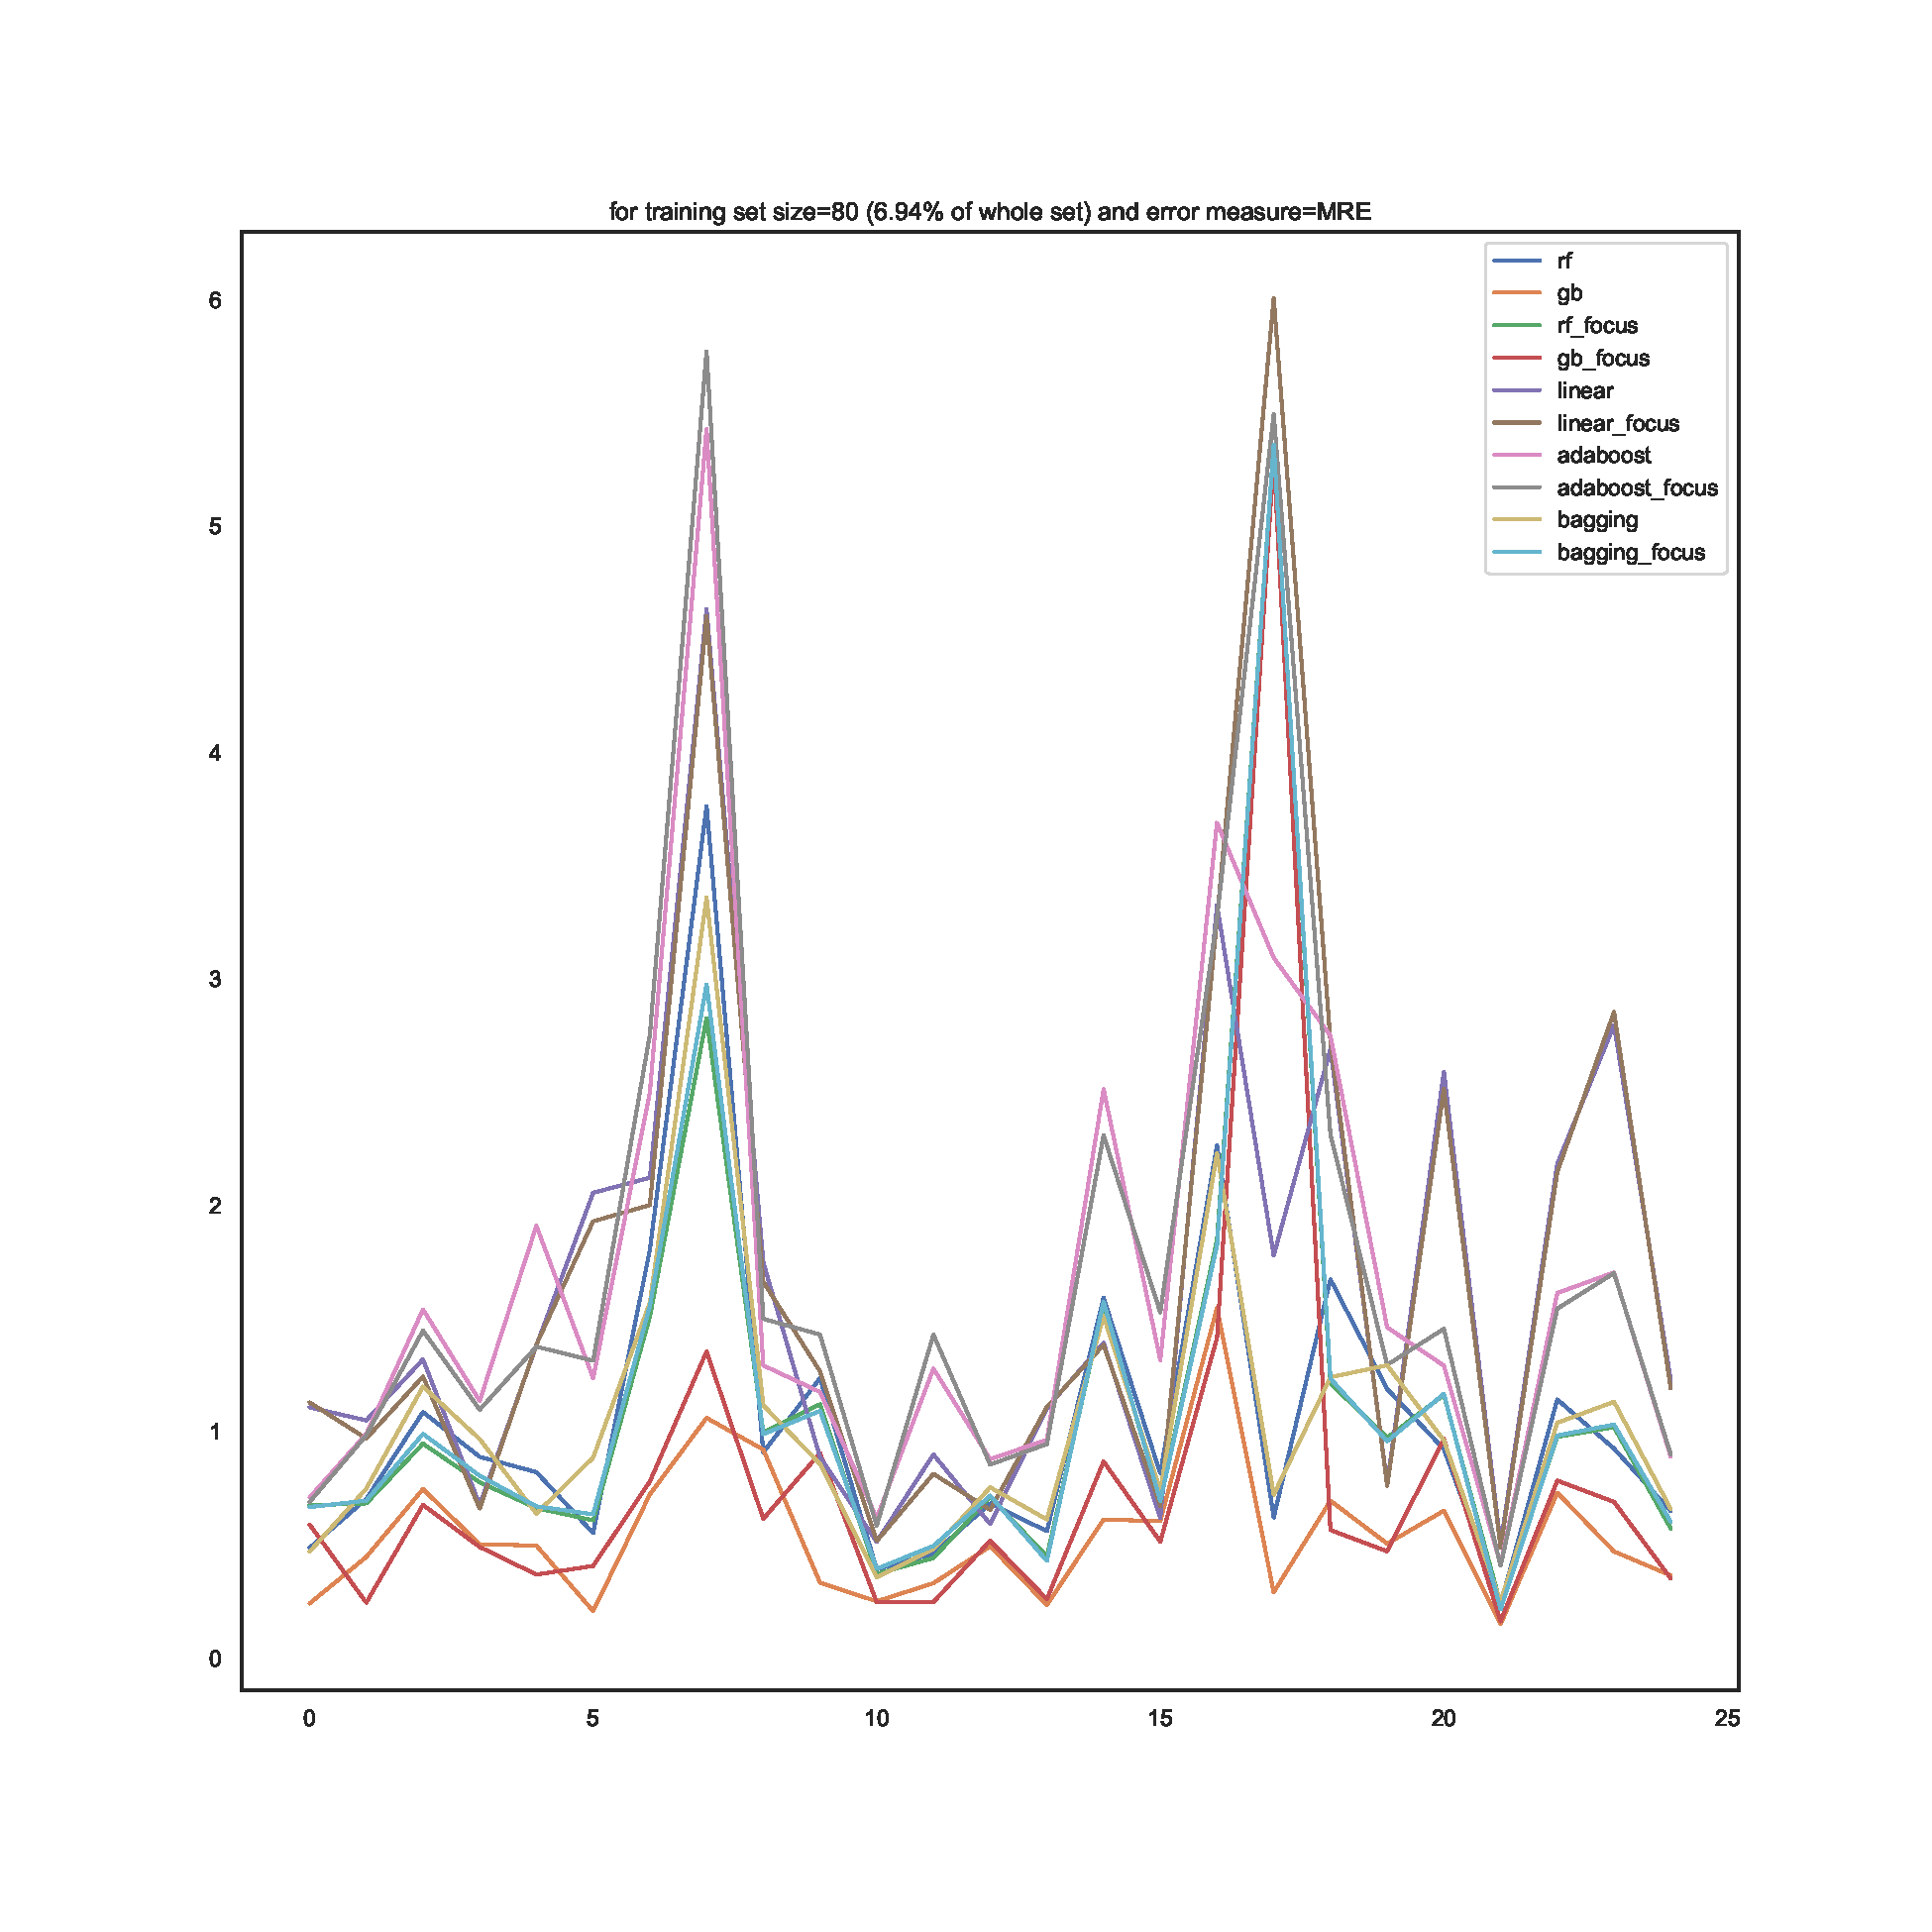
\includegraphics[scale=0.12]{JupyterImages/focuseffect_evo_80_MRE-size.pdf}}
\subfloat[\label{fig:accuracy-mlalgos-time112} N=112]{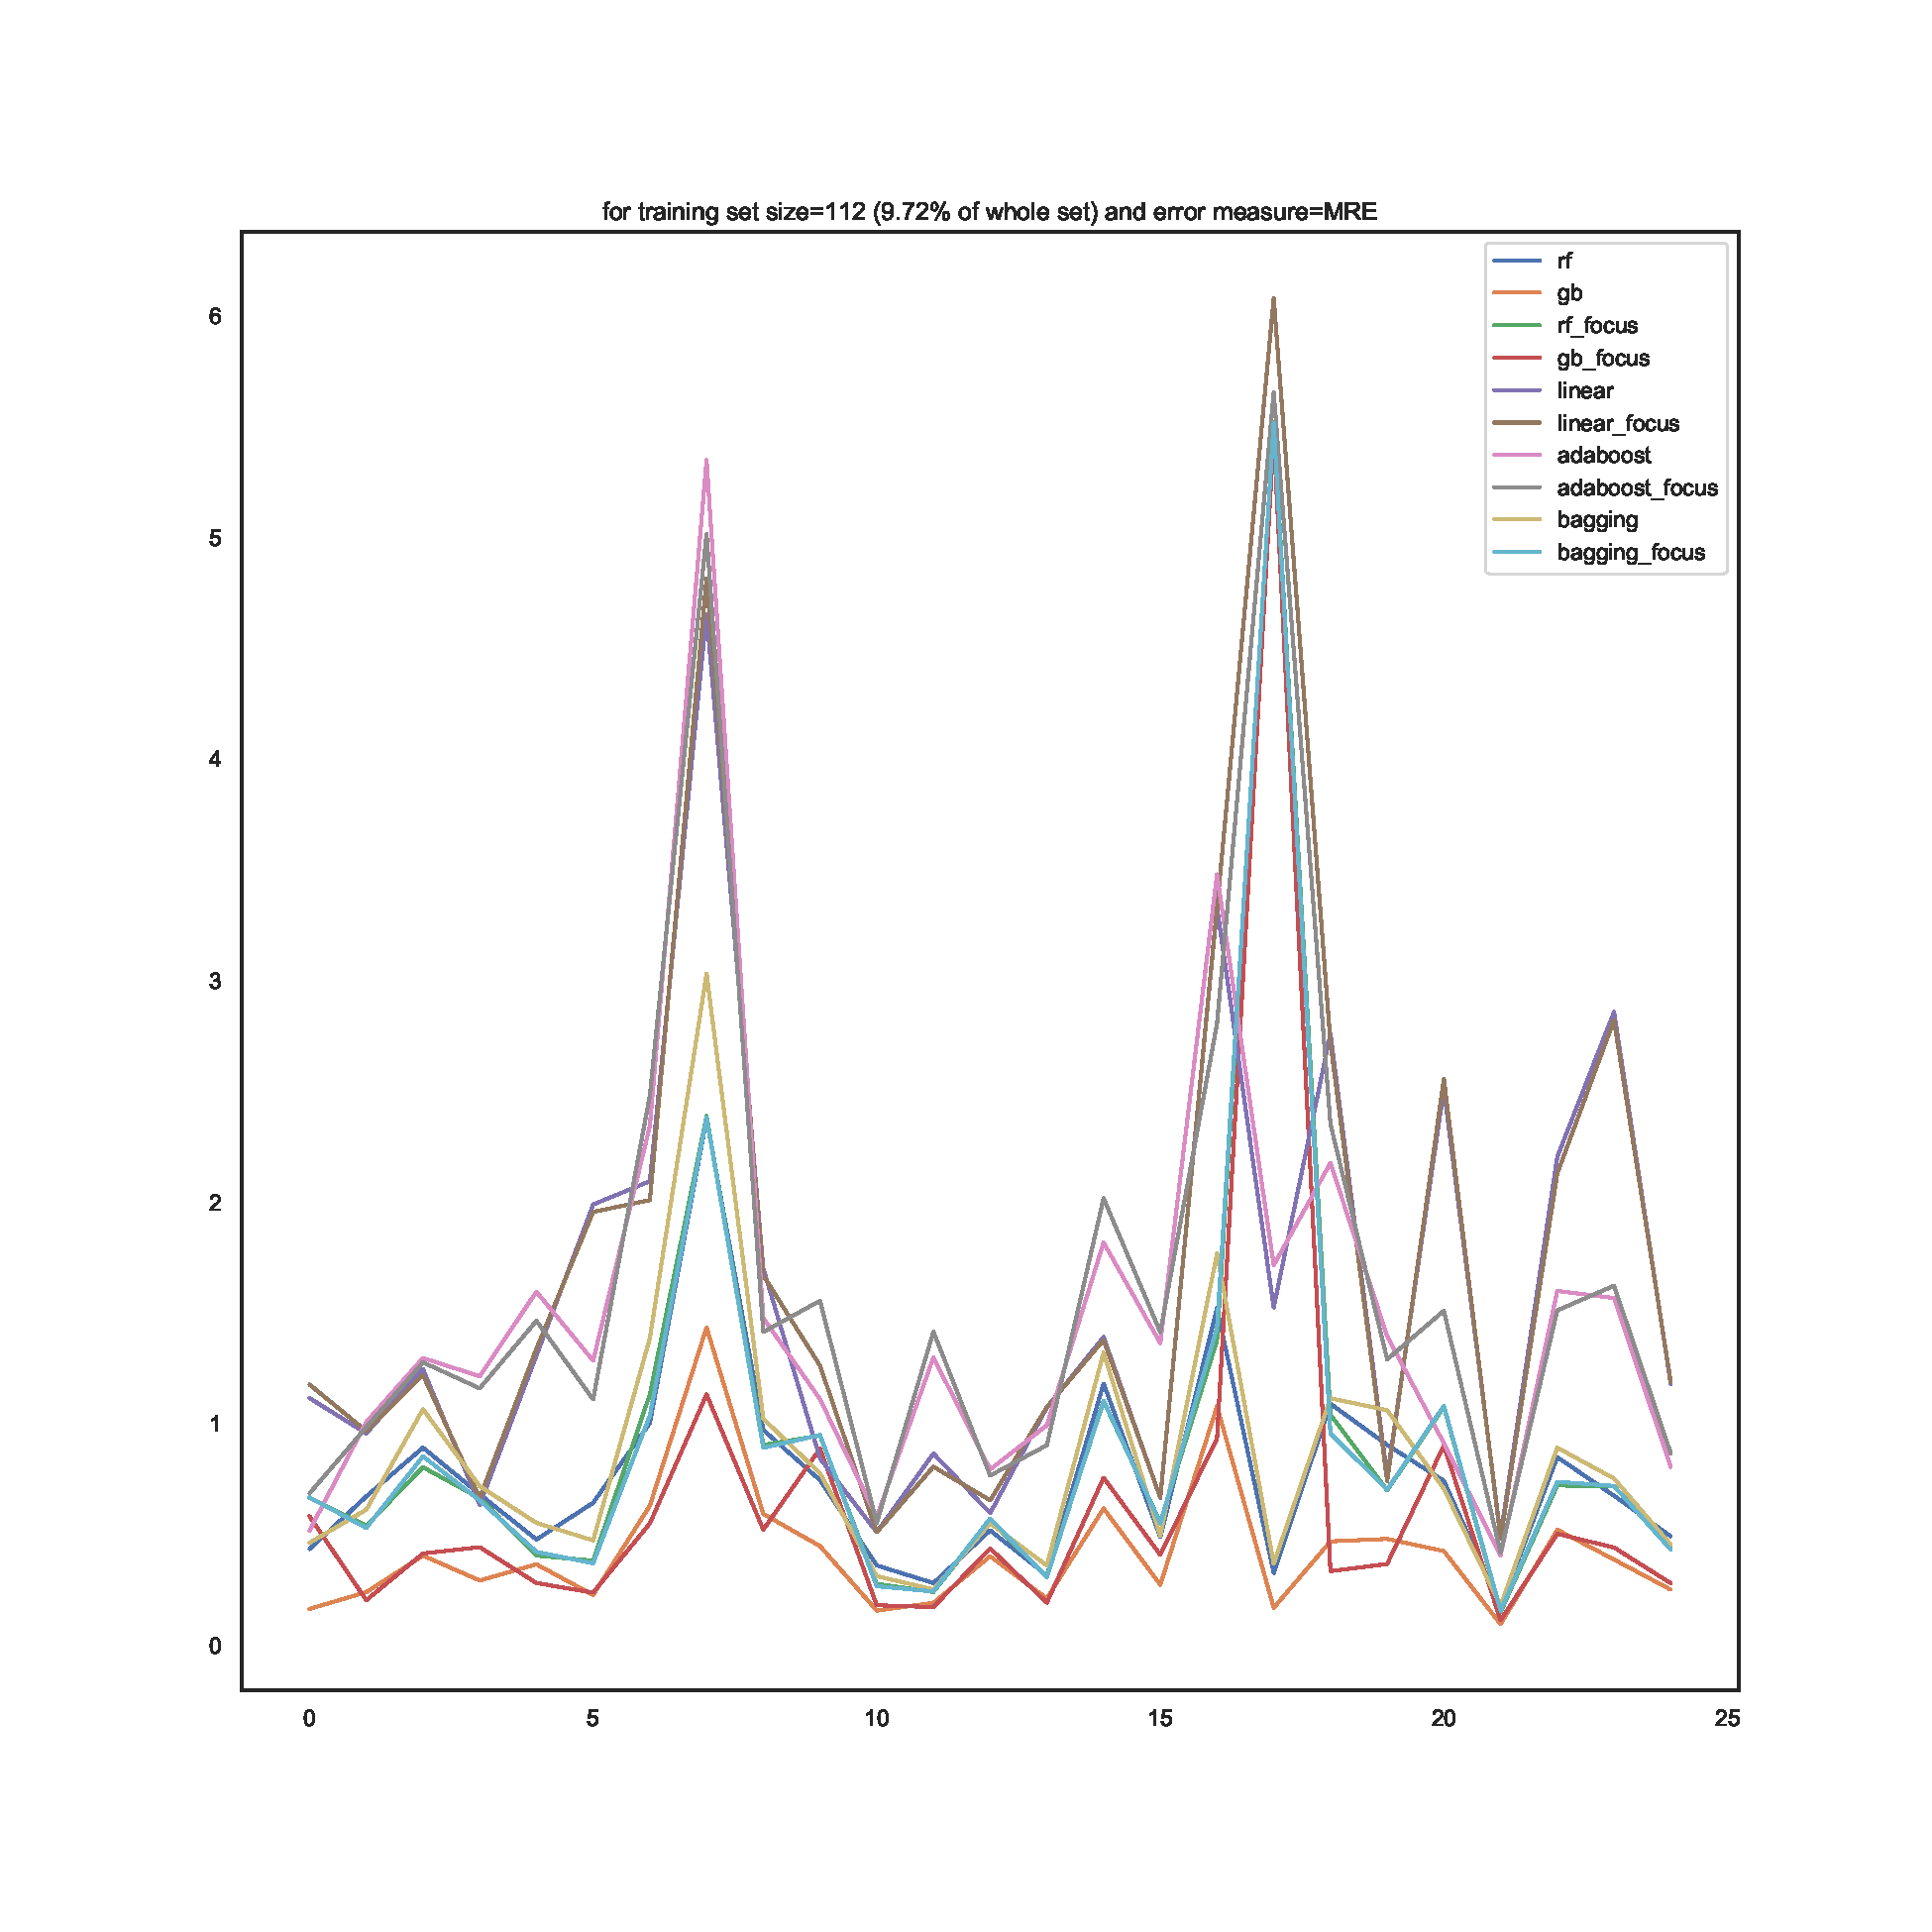
\includegraphics[scale=0.12]{JupyterImages/focuseffect_evo_112_MRE-size.pdf}}\\
\subfloat[\label{fig:accuracy-mlalgos-time160} N=160]{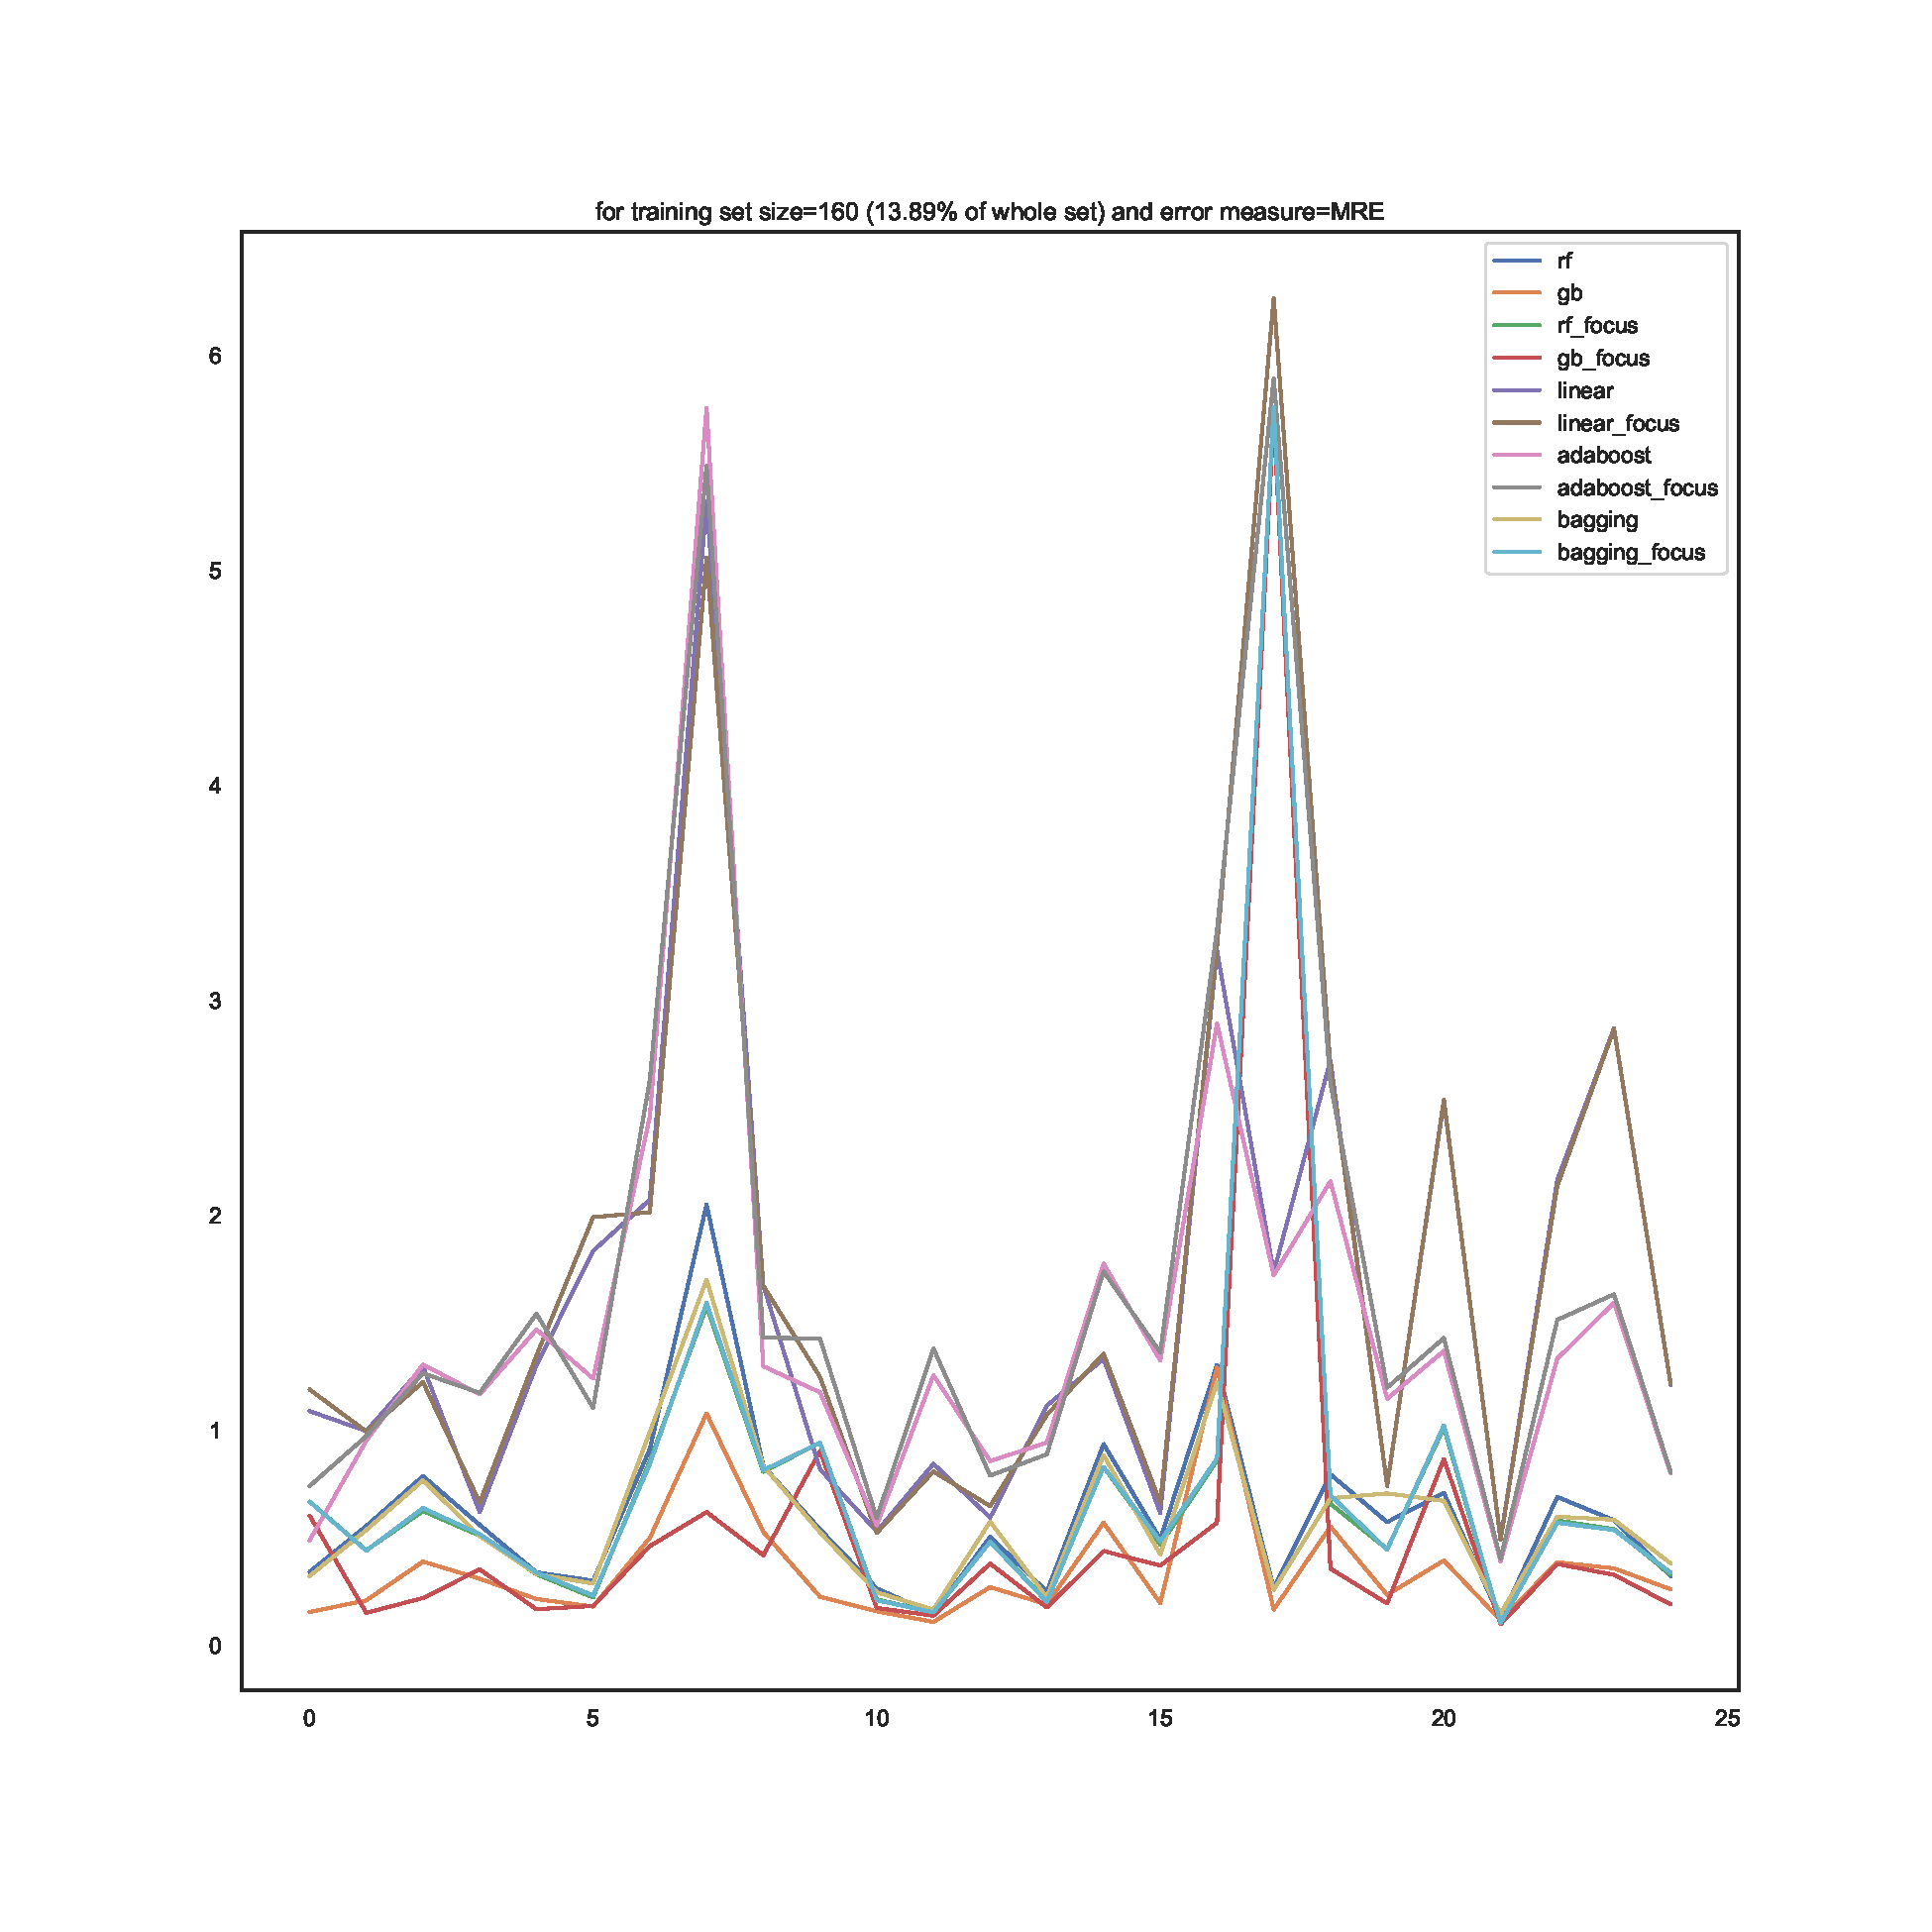
\includegraphics[scale=0.12]{JupyterImages/focuseffect_evo_160_MRE-size.pdf}}
\subfloat[\label{fig:accuracy-mlalgos-time240} N=240]{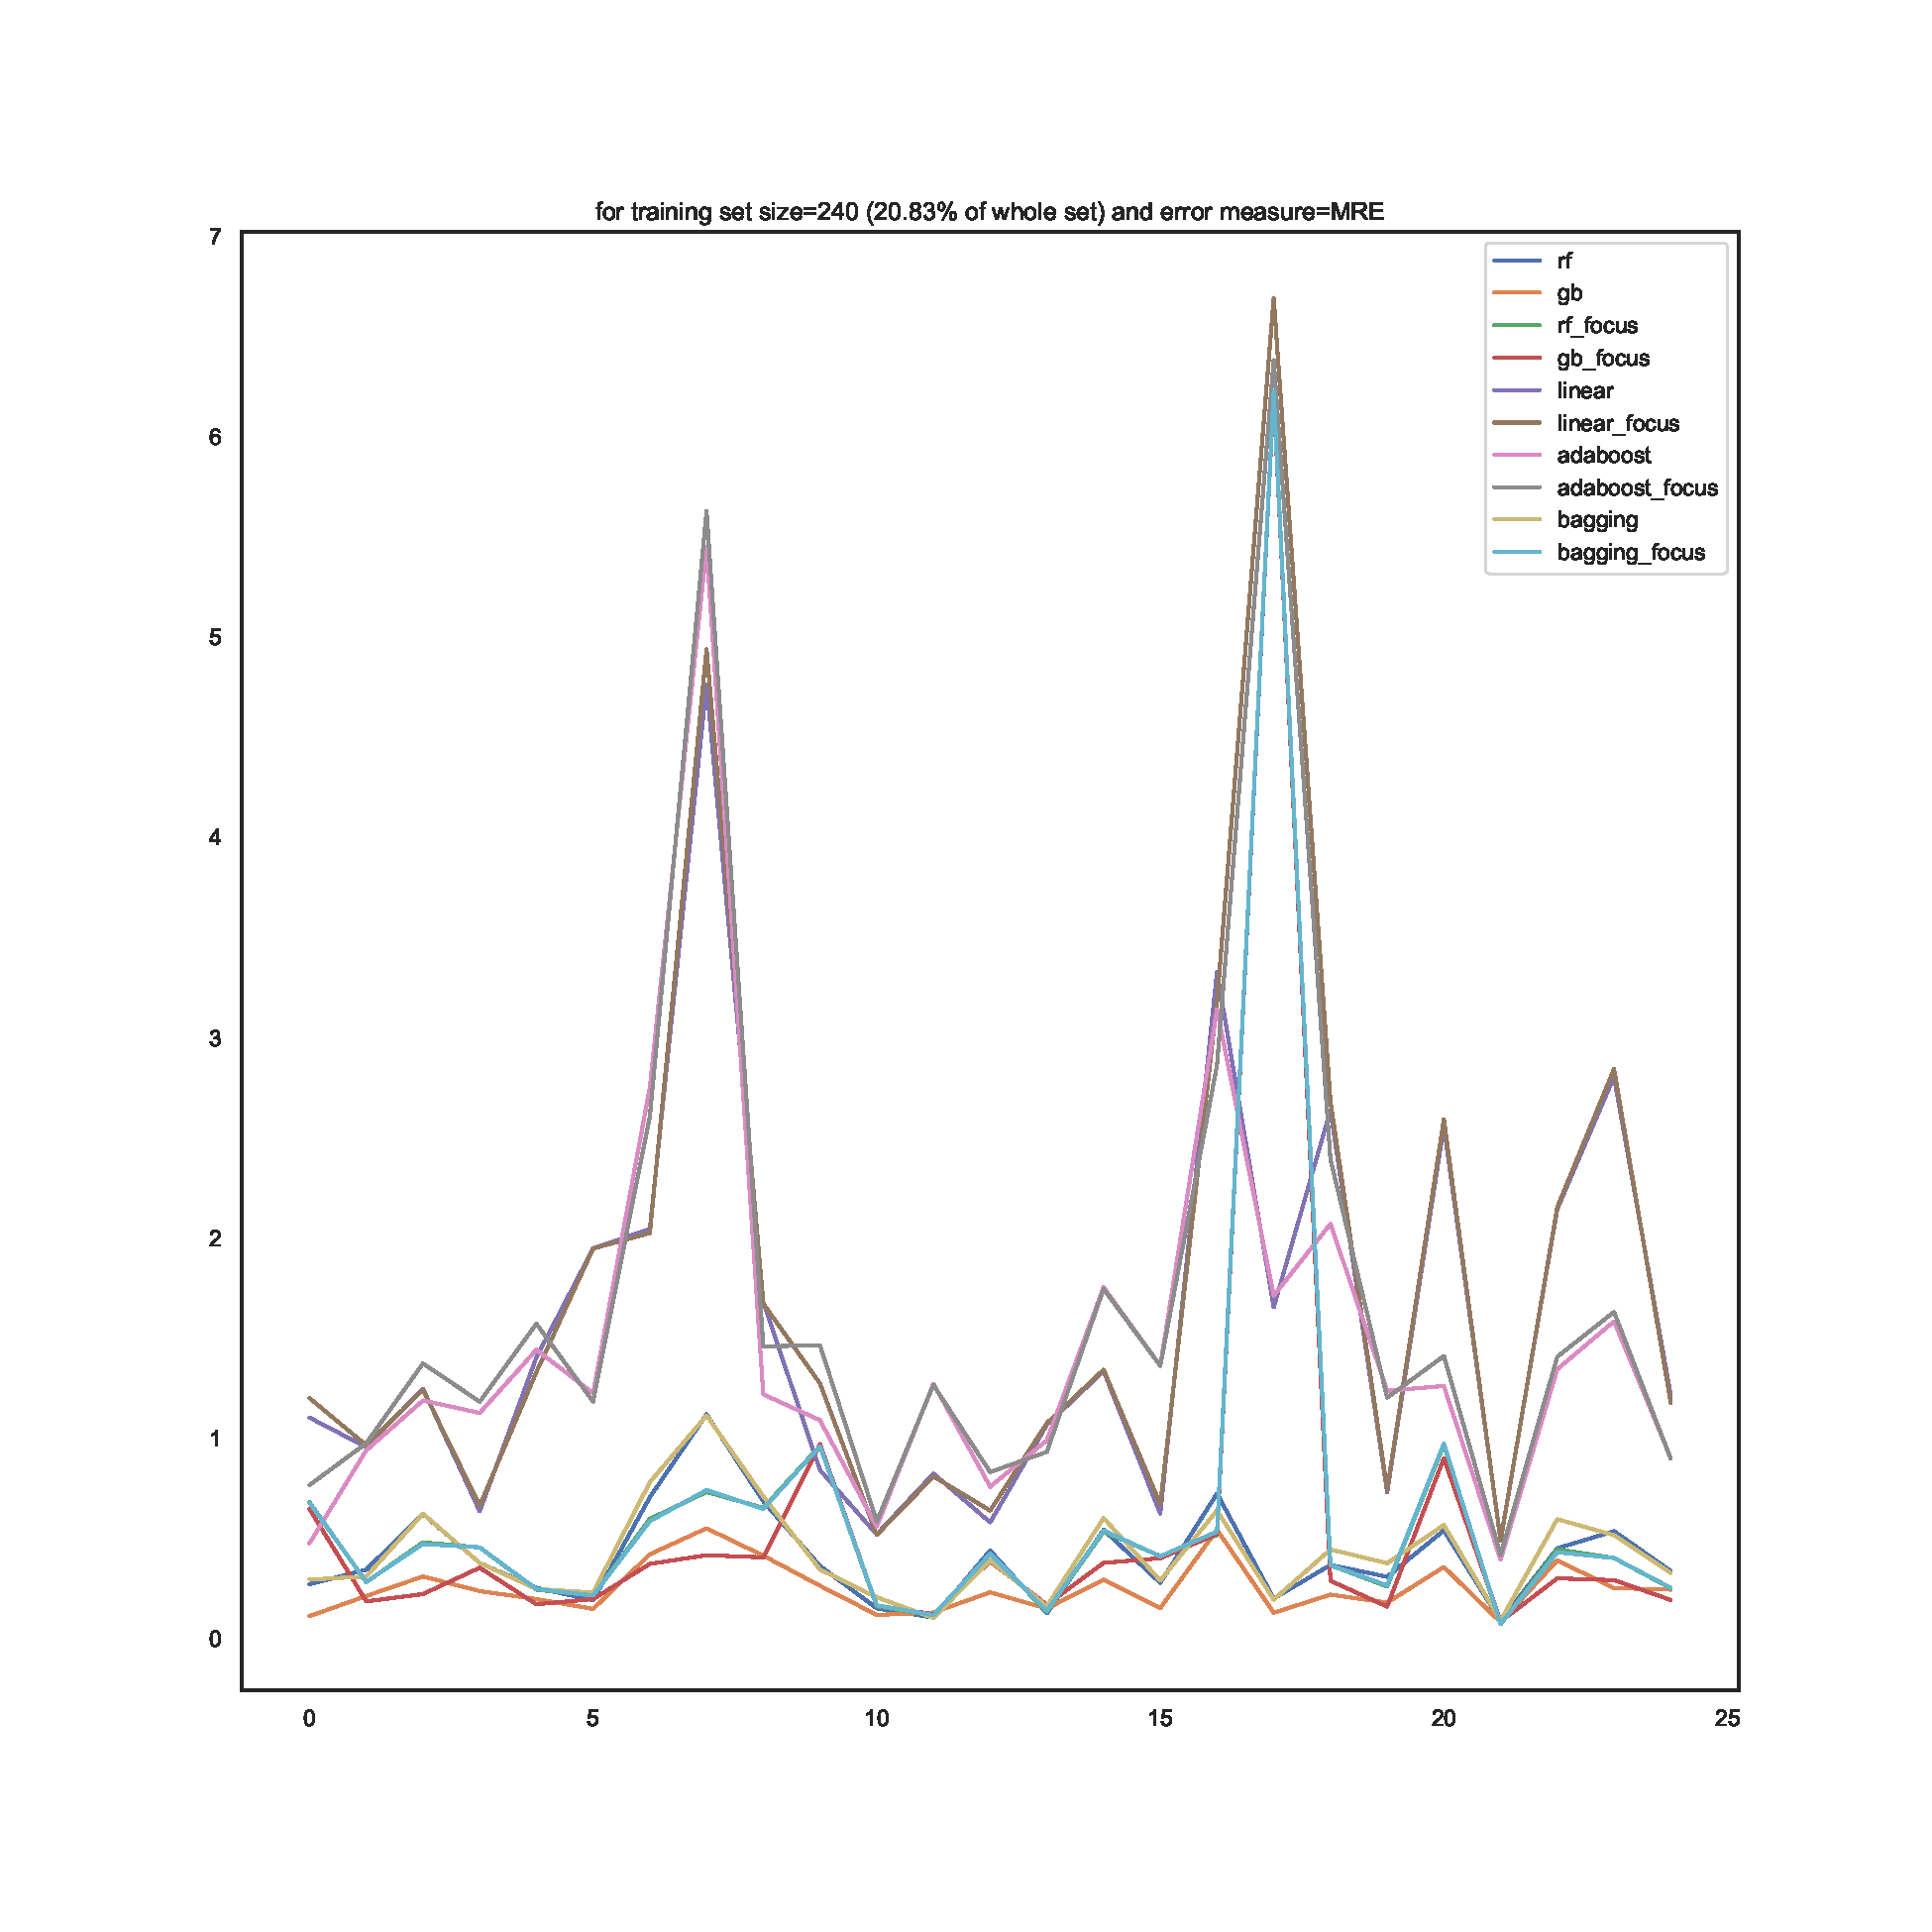
\includegraphics[scale=0.12]{JupyterImages/focuseffect_evo_240_MRE-size.pdf}}\\
\caption[caption]{\label{fig:accuracy-mlalgos-size-matrices}Learning results (size) of learning algorithms, with and without K2R sampling; N is the size of the training set}\end{figure*}\begin{figure}\centering
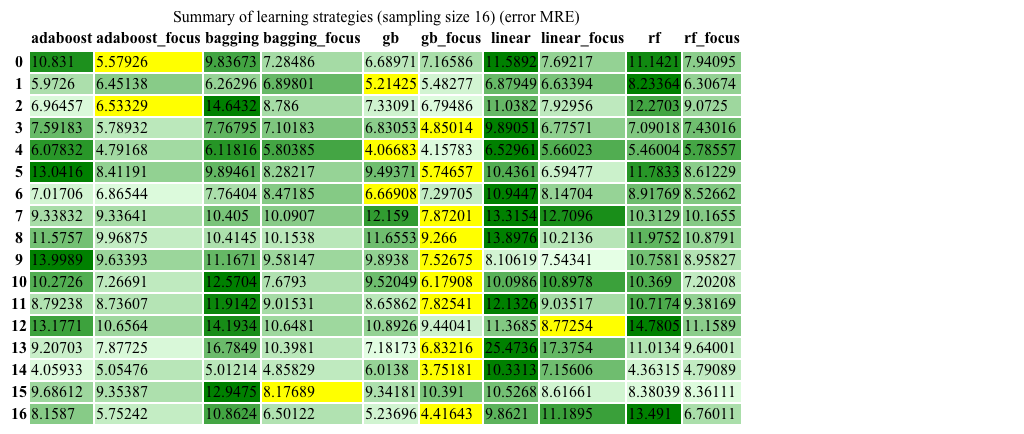
\includegraphics[scale=0.28]{JupyterImages/focuseffect_16_MRE-elapsedtime.png}\caption{\label{tab:accuracy-mlalgos-matrix-time16} Learning results (size) of learning algorithms, with and without K2R sampling; N=16 is the size of the training set}\end{figure}\begin{figure}\centering
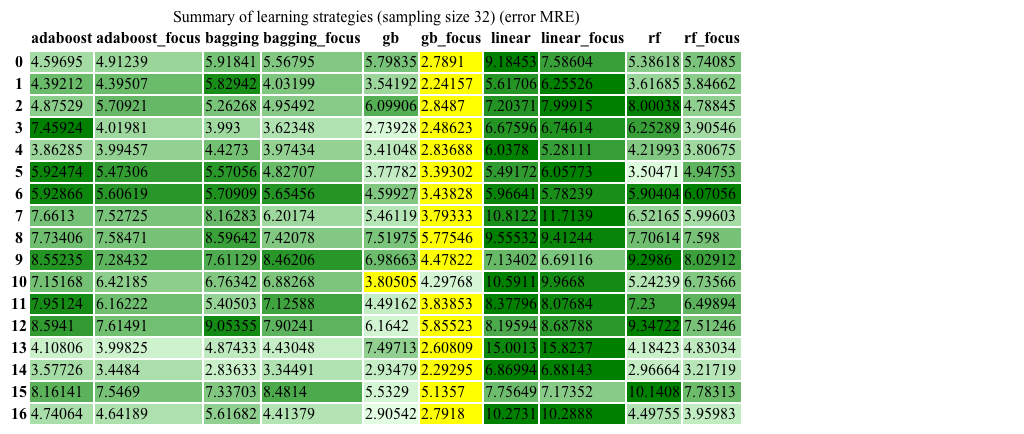
\includegraphics[scale=0.28]{JupyterImages/focuseffect_32_MRE-elapsedtime.png}\caption{\label{tab:accuracy-mlalgos-matrix-time32} Learning results (size) of learning algorithms, with and without K2R sampling; N=32 is the size of the training set}\end{figure}\begin{figure}\centering
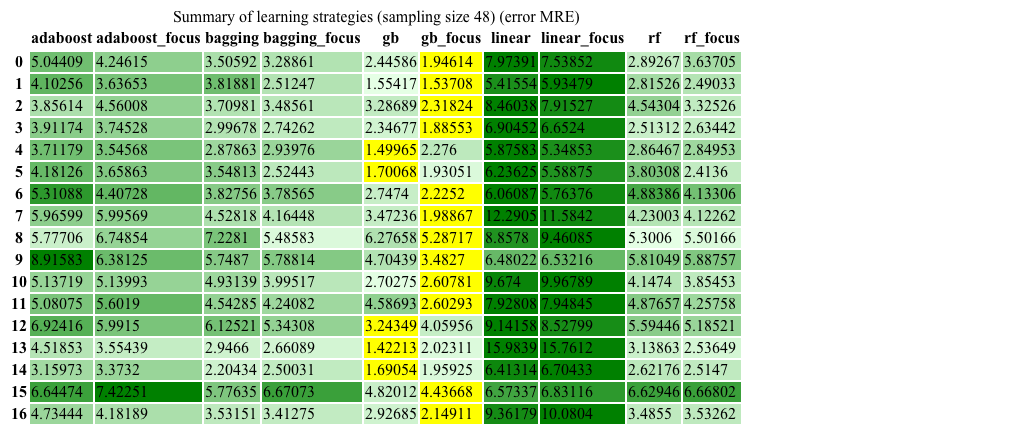
\includegraphics[scale=0.28]{JupyterImages/focuseffect_48_MRE-elapsedtime.png}\caption{\label{tab:accuracy-mlalgos-matrix-time48} Learning results (size) of learning algorithms, with and without K2R sampling; N=48 is the size of the training set}\end{figure}\begin{figure}\centering
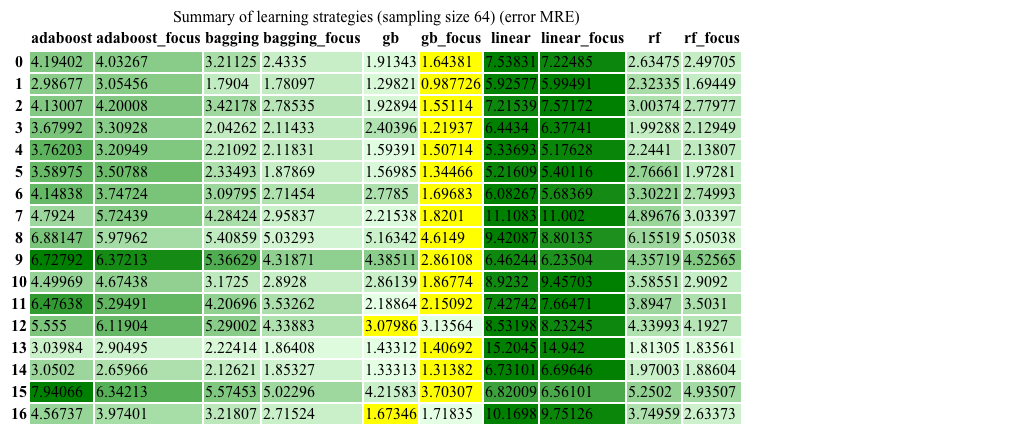
\includegraphics[scale=0.28]{JupyterImages/focuseffect_64_MRE-elapsedtime.png}\caption{\label{tab:accuracy-mlalgos-matrix-time64} Learning results (size) of learning algorithms, with and without K2R sampling; N=64 is the size of the training set}\end{figure}\begin{figure}\centering
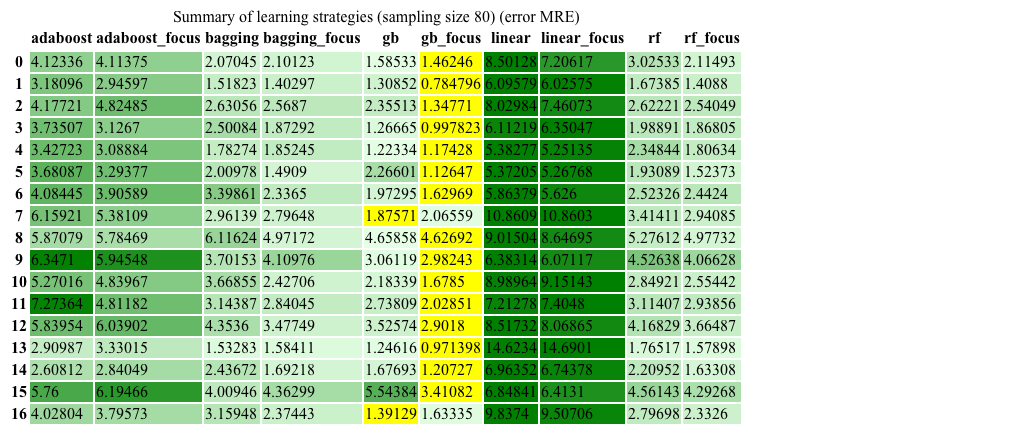
\includegraphics[scale=0.28]{JupyterImages/focuseffect_80_MRE-elapsedtime.png}\caption{\label{tab:accuracy-mlalgos-matrix-time80} Learning results (size) of learning algorithms, with and without K2R sampling; N=80 is the size of the training set}\end{figure}\begin{figure}\centering
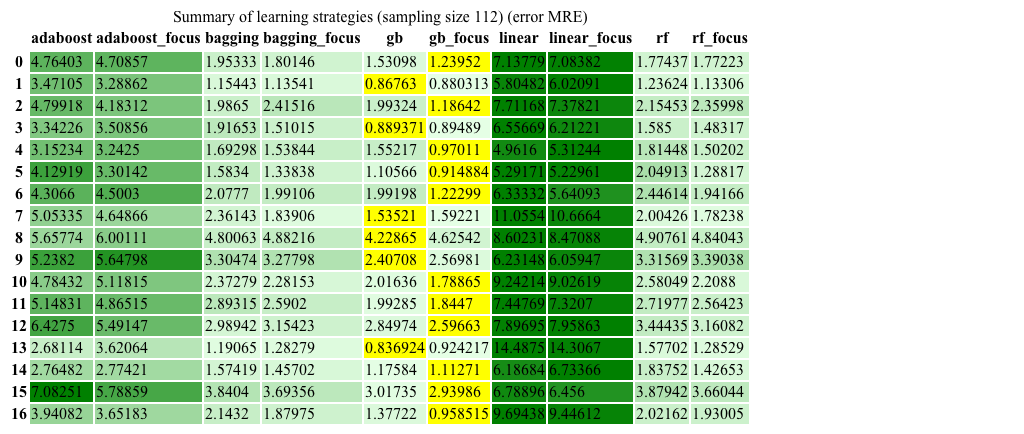
\includegraphics[scale=0.28]{JupyterImages/focuseffect_112_MRE-elapsedtime.png}\caption{\label{tab:accuracy-mlalgos-matrix-time112} Learning results (size) of learning algorithms, with and without K2R sampling; N=112 is the size of the training set}\end{figure}\begin{figure}\centering
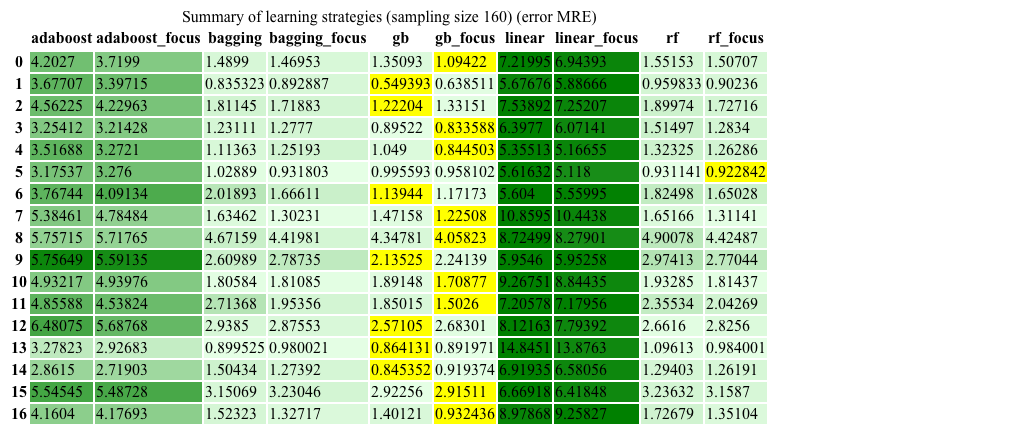
\includegraphics[scale=0.28]{JupyterImages/focuseffect_160_MRE-elapsedtime.png}\caption{\label{tab:accuracy-mlalgos-matrix-time160} Learning results (size) of learning algorithms, with and without K2R sampling; N=160 is the size of the training set}\end{figure}\begin{figure}\centering
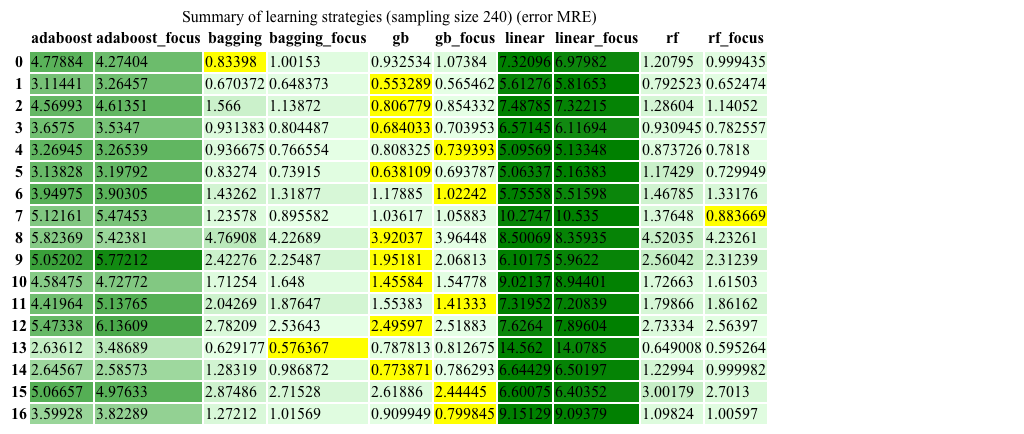
\includegraphics[scale=0.28]{JupyterImages/focuseffect_240_MRE-elapsedtime.png}\caption{\label{tab:accuracy-mlalgos-matrix-time240} Learning results (size) of learning algorithms, with and without K2R sampling; N=240 is the size of the training set}\end{figure}